%!TEX root = main.tex

%We have defined the formal semantics of {\AMASS} models defined in Section~\ref{sec:amass}. 

The goal of this section is to validate the formal semantics of the {\AMASS} models defined in Section~\ref{sec:amass}.  
%to justify its correctness. 
To avoid tediousness, we focus on the two sub-models $\AOAMASS$ and $\FOAMASS$ of {\AMASS} %. Moreover, we focus on the validation of the formal semantics for 
and Android 13.0. 
%
We validate the formal semantics from two different perspectives. 
\begin{itemize}
\item At first, we audit the Java source code of Android operating system to extract the control flows of starting an activity and executing a fragment transaction respectively. We confirm that the formal semantics of {\AMASS} models defined in Section~\ref{sec:amass} indeed echo the extracted control flows. See Section~\ref{sec:val-code} for more about the code audit. 
%
\item Moreover, we select 21 Android apps to empirically validate the conformance of the formal semantics of {\AMASS} models to the actual behaviors of these apps in the Android operating system. The details of the empirical validation are given in Section~\ref{sec:val-exp}. 
\end{itemize}

%Recall that in Section~\ref{sec:amass}, we separate the concerns and define the semantics for the sub-models $\AOAMASS$ and $\FOAMASS$ and put the definition of the semantics of {\AMASS} in the appendix. To be consistent with the definition of the semantics, in the sequel, we show how to validate the semantics for $\AOAMASS$ and $\FOAMASS$ models, and put the validation of the semantics for {\AMASS} models in Appendix~\ref{app-sem-val-amass}. 

\subsection{Validation of the formal semantics by auditing the source code of Android OS}\label{sec:val-code}
%
%To validate the formal semantics by reviewing the Android source code, we only consider the two sub-models $\AOAMASS$ and $\FOAMASS$. 
%Since the Android source code is complicated, and the validation of the formal semantics of $\AOAMASS$ and $\FOAMASS$ is highly complicated. 
To validate the formal semantics of $\AOAMASS$ (resp. $\FOAMASS$), we audit the source code of Android OS. Specifically, we trace the control flow of the Java source code\footnote{available at \url{https://android.googlesource.com/platform/frameworks/base/}.} starting from the procedure startActivity() (resp. commit()). %We focus on Android 13.0. 
\revision{To increase the quality of the auditing process, we audit the source code in two phases. In the first phase, the three authors audit the relevant parts of the source code of Android OS separately.  Then in the second phase, the three authors have a joint discussion and achieve a consensus on the understanding of the source code.}

%The source code are shown in Appendix~\ref{app:code-audit}.
We first consider $\AOAMASS$, then $\FOAMASS$. 
%Similarly, we trace the control flow when the procedure commit() is called to validate 
%To validate the formal semantics of $\AOAMASS$, we start from the function startActivity(), and trace the calls of functions, finally check whether the behavior of the back stack is consistent with the formal semantics. 
%Similarly, to validate the semantics of $\FOAMASS$, we start from the function commit(), finally check whether the behavior of the fragment stack and fragment transaction stack is consistent with the formal semantics.
%

\subsubsection{Auditing the source code of $\AOAMASS$}
Figure~\ref{fig:startActivity} shows the control flow starting from the procedure startactivity() in the Activity class, 
where the vertices represent the procedures in classes and edges represent the procedure calls. 

\begin{itemize}
\item Starting from startactivity(),  startActivityForResult() is called, then execStartActivity() is called, and so on, until the procedure startActivityInner() is reached, where the core control logic for starting an activity is implemented. 
%
\item In the procedure startActivityInner(), the following statements are executed sequentially: the procedure computeLaunchingTaskFlags(), a conditional statement where getReusableTask() and computeTargetTask() are in the two branches respectively, the procedure recycleTask(), and another conditional statement where setNewTask() and addOrReparentStartingActivity() are in the two branches respectively.  
%
\item The procedure getReusableTask() calls findTask(), in which the procedure process() is called, and process() calls the procedure forAllLeafTasks(), where the procedure test() is called. 
%
\item The procedure recycleTask() calls the procedure complyActivityFlags() and setNewTask() calls reuseOrCreateTask() respectively.
\end{itemize}
%\hide{
%    \begin{itemize}
%        \item in the Activity.java file, startActivity() function calls startActivityForResult() function in line 6043, then startActivityForResult() function calls execStartActivity() function of Instrumentation class in 6423,
%        \item in the Instrumentation.java file, execStartActivity() function calls startActivity() function of ActivityTaskManagerService class in line 1873,
%        \item in the ActivityTaskManagerService.java file, startActivity() function calls startActivityAsUser() function in line 1214, then startActivityAsUser() function calls execute() function in line 1288, we can see that execute() is a function of ActivityStarter class via line 1276 in ActivityTaskManagerService.java file and line 133 to line 135 in ActivityStartController.java file,
%        \item in the ActivityStarter.java file, execute() function calls executeRequest() function in line 742, and executeRequest() function calls startActivityUnchecked() function in line 1309, finally startActivityUnchecked() func calls startActivityInner() function in line 1479.
%    \end{itemize}
%}
\begin{figure}[htbp]
    % \vspace{-3mm}
        \centering
        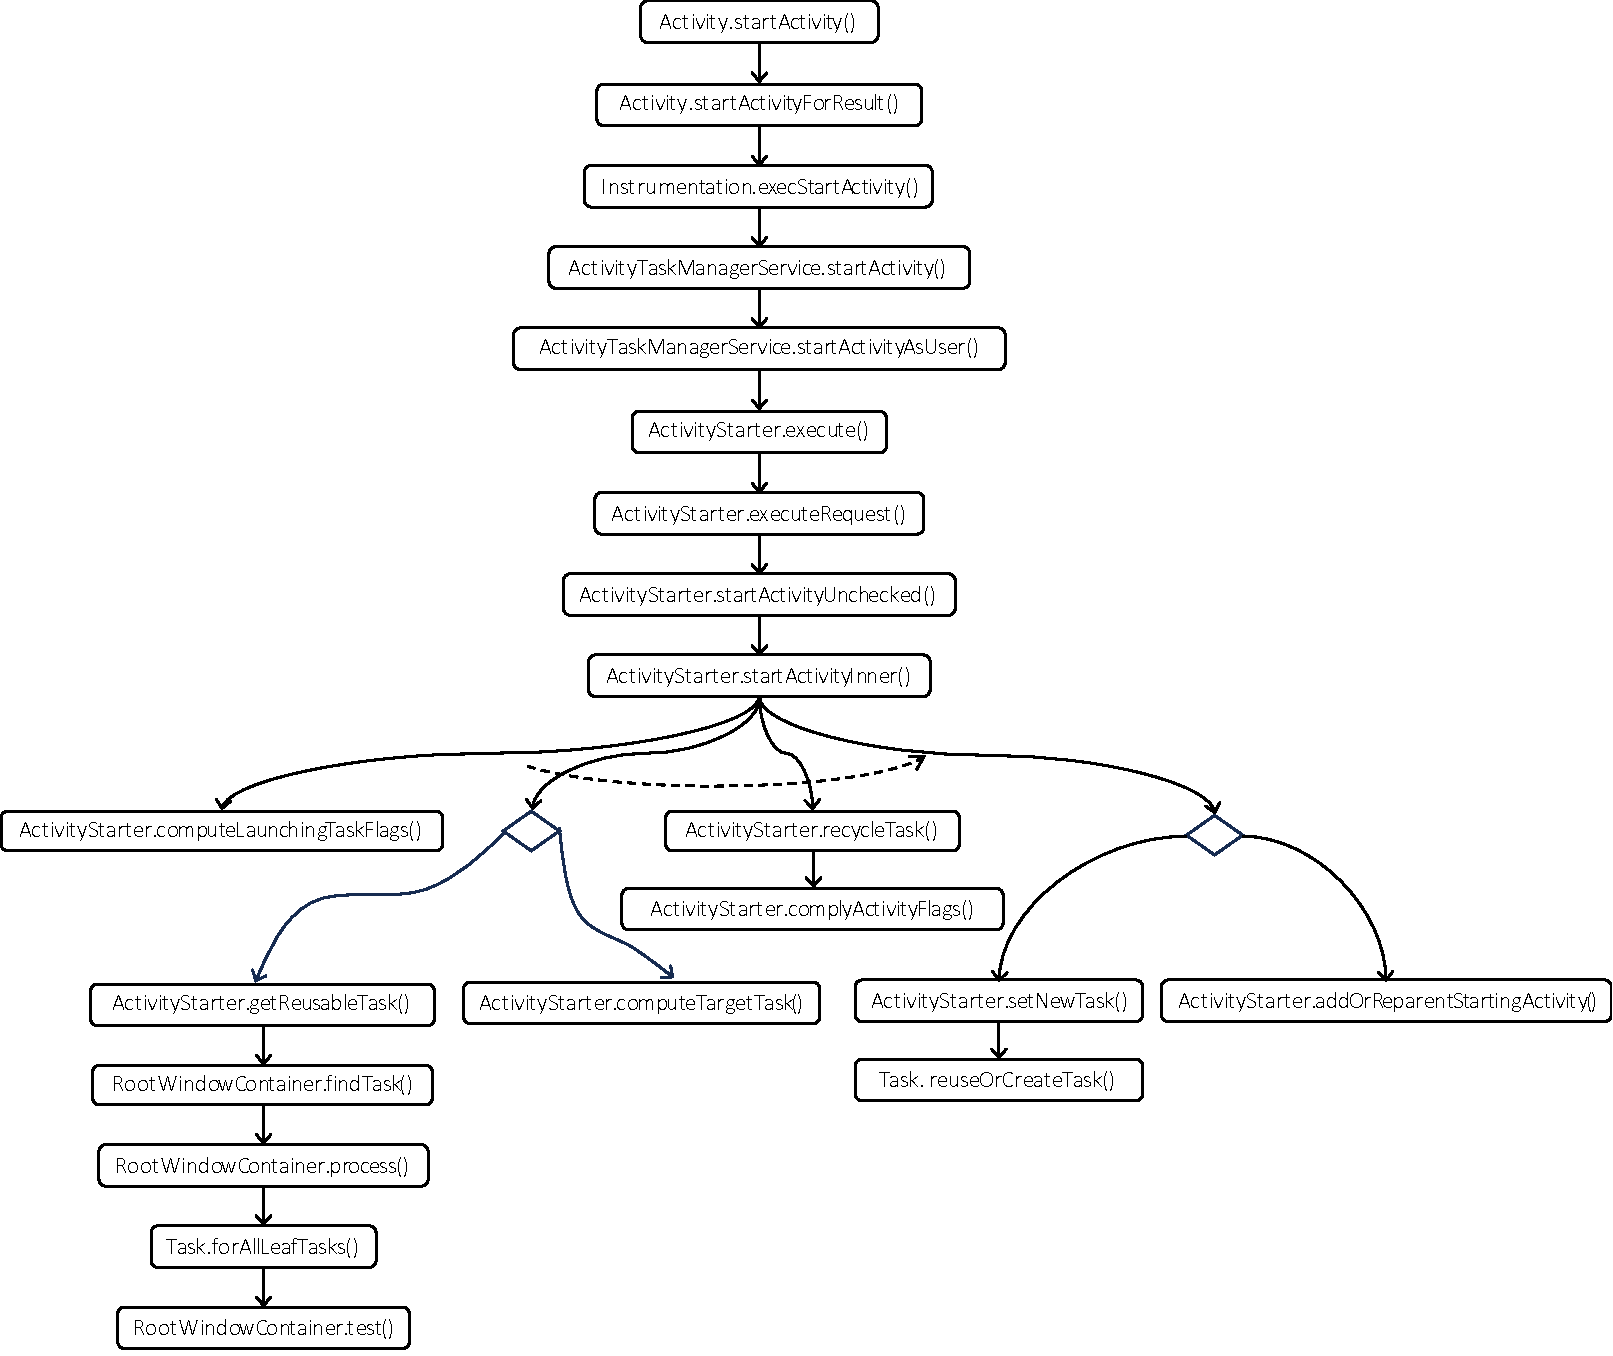
\includegraphics[scale = 0.55]{startActivity.pdf}
        \caption{Call graph for starting an activity}
            %in $\phi$
    % \vspace{-6mm}	
    \label{fig:startActivity}
\end{figure}

We audit the source code of the procedures called directly or indirectly by startActivityInner() and confirm that the semantics of $\AOAMASS$ is consistent with its actual implementation in Android OS. In particular, the task allocation mechanism and the intent flags in the semantics conform to the source code in Android OS.
The details of the auditing are relegated to Appendix~\ref{app:code-audit-aomass}. 

%%%%%%%%% the original text by Jinlong %%%%%%%
%%%%%%%%% the original text by Jinlong %%%%%%%
\hide{
Then it will call recycleTask() function in line 1716 to place $B$.
As shown in Code~\ref{code-recycleTask}, recycleTask() function actually calls complyActivityFlags() function in line 2090 to place $B$ in the task with the actual intent flags. 

    Recall that the formal semantics of $\AOAMASS$, there are three main steps for the evolution of the task stack by starting an activity $B$ from an activity $A$ as follows:
    \begin{enumerate}
        \item It will search for a task for $B$ according to the task allocation mechanism.
        \item Then it will place the activity $B$ in that task according to the intent flags, and the launch modes of $A$ and $B$,
    \end{enumerate}

\begin{itemize}
    \item As shown in Code~\ref{code-getReusableTask}, the getReusableTask() function in the ActivityStarter.java file will call findTask() function in line 2883 to search for a reusable task for the caller activity $B$. For each task in the task stack, findTask() will call test() function to check whether it is the target task. The test() function in the RootWindowContainer.java file will first check whether the real activity of the task matches the caller activity $B$ in line 392 (corresponding to the first step), then check whether the task affinity of the task matches the task affinity of the caller activity $B$ in line 399 (corresponding to the second step). 
    \item As shown in Code~\ref{code-setNewTask}, the setNewTask() function in the ActivityStarter.java file will create a new task for $B$ in line 3054(corresponding to the last step).
\end{itemize}



%search for a reusable target task in the task stack for the caller activity by calling getReusableTask() in line 1652 (corresponding to the first step) first. 
Then it will place the caller activity in the target task by calling recycleTask() in line 1709 (corresponding to the second step). 
    % Finally, if no such reusable task found, it will call setNewTask() in line 1734 to create a new task for the caller activity. Moreover, 

    Furthermore, recall that the task allocation mechanism, there are three steps:
    \begin{enumerate}
        \item If there is any task whose real activity is $B$, then $B$ will be put on the task. %(search downwards from the top task). 
        \item Otherwise, if there is any task whose real activity has the same \emph{task affinity} as $B$, then $B$ will be put on the task. %first such task (search downwards from the top task). 
        \item Otherwise, a new task is created to hold $B$. 
    \end{enumerate}
        In the first two steps, if there are multiple instances, the first occurrence starting from the top task will be selected. 
We confirm the task allocation mechanism by reviewing Code~\ref{code-getReusableTask} (corresponding to the first two steps) and Code~\ref{code-setNewTask} (corresponding to the last step). Moreover.
\begin{itemize}
    \item As shown in Code~\ref{code-getReusableTask}, the getReusableTask() function in the ActivityStarter.java file will call findTask() function in line 2883 to search for a reusable task for the caller activity $B$. For each task in the task stack, findTask() will call test() function to check whether it is the target task. The test() function in the RootWindowContainer.java file will first check whether the real activity of the task matches the caller activity $B$ in line 392 (corresponding to the first step), then check whether the task affinity of the task matches the task affinity of the caller activity $B$ in line 399 (corresponding to the second step). 
    \item As shown in Code~\ref{code-setNewTask}, the setNewTask() function in the ActivityStarter.java file will create a new task for $B$ in line 3054(corresponding to the last step).
\end{itemize}
% Finally, if no such reusable task found, getReusableTask() function will call setNewTask() function in line 1734, as shown in Code~\ref{code-setNewTask}, setNewTask() function will create a new task for the caller activity $B$ in line 3054 (corresponding to the third step).

Indeed, the combination of intent flag and launch modes of $A$ and $B$ has a collective impact on the placement of $B$. As shown in Code~\ref{code-startActivityInner}, startActivityInner() function will call the computeLaunchingTaskFlags() function in line 1636 to compute the actual intent flags via converting the launch modes to the intent flags. Then it will call recycleTask() function in line 1709 to place $B$.
As shown in Code~\ref{code-recycleTask}, recycleTask() function actually calls complyActivityFlags() function in line 2236 to place $B$ in the task with the actual intent flags. Moreover, recall that there are 4 ways to place $B$, i.e., $\clrtsk(\rho, B)$, $\clrtop(\rho, B)$, $\mvacttop(\rho, B)$ and $\push(\rho, B)$. The details of complyActivityFlags() function are shown as follows:
\begin{itemize}
    \item it will clear all activities in the task in line 2402 and push the caller activity $B$ into the task in line 2404 (corresponding to $\clrtsk(\rho, B)$),
    \item it will clear all activities above the caller activity $B$ in line 2414 (corresponding to $\clrtop(\rho, B)$),
    \item it will move the caller activity $B$ to the top of the task in line 2458 (corresponding to $\mvacttop(\rho, B)$),
    \item it will push the caller activity $B$ into the task directly in line 2495 (corresponding to $\push(\rho, B)$).
\end{itemize}

%
%    We confirm the behavior of the back stack is consistent with our formal semantics of $\AOAMASS$ defined in Section~\ref{sec:aoamass} by reviewing the Android source code. As shown in Code~\ref{scode-startActivity}, startActivity() function is involved to start an activity $B$ from $A$, 
%
    \begin{itemize}
        \item in the Activity.java file, startActivity() function calls startActivityForResult() function in line 6043, then startActivityForResult() function calls execStartActivity() function of Instrumentation class in 6423,
        \item in the Instrumentation.java file, execStartActivity() function calls startActivity() function of ActivityTaskManagerService class in line 1873,
        \item in the ActivityTaskManagerService.java file, startActivity() function calls startActivityAsUser() function in line 1214, then startActivityAsUser() function calls execute() function in line 1288, we can see that execute() is a function of ActivityStarter class via line 1276 in ActivityTaskManagerService.java file and line 133 to line 135 in ActivityStartController.java file,
        \item in the ActivityStarter.java file, execute() function calls executeRequest() function in line 742, and executeRequest() function calls startActivityUnchecked() function in line 1309, finally startActivityUnchecked() func calls startActivityInner() function in line 1479.
    \end{itemize}
    Consequently, startActivityInner() function in the ActivityStarter.java file deals with how to start $B$ in the back stack, the codes of startActivityInner() function are shown in Code~\ref{code-startActivityInner}.


Therefore, through reviewing Android source code, we discover that the behavior of the back stack shown in the source code is essentially consistent with the formal semantics of $\AOAMASS$.


% \begin{itemize}
% 	\item As shown in Code~\ref{code-getReusableTask}, 
%     getReusableTask() function will call findTask() function in line 2883 to search for a reusable task for the caller activity. For each task in the task stack, findTask() will call test() function shown in Code~\ref{code-test} to check whether it is the target task. 
% 	\item As shown in Code~\ref{code-recycleTask}, recycleTask() function will call complyActivityFlags() in line 2236 to place the caller activity in the target task. As shown in Code~\ref{code-complyActivityFlags}, complyActivityFlags() function will clear all activities in the target task and push the caller activity into the task in line 2420, or clear all activities above the caller activity in line 2432, or move the caller activity to the top of the target task in line 2474, or push the caller activity into the target task directly in line 2500, according to the launch modes of callee activity and caller activity, and the intent flags.
% 	\item As shown in Code~\ref{code-setNewTask}, setNewTask() function will create a task for the caller activity in line 3054.
% \end{itemize}
%\begin{lstlisting}[caption={The sample code for startActivity()},label={scode-startActivity}]
%    Intent intent = new Intent(A.this, B.class);
%    intent.setFlags(Intent.FLAG_ACTIVITY_NEW_TASK);
%    startActivity(intent);
%\end{lstlisting}

\begin{figure}[htbp]
\centering
\begin{tabular}{c}
%[basicstyle=\footnotesize\ttfamily]
\begin{lstlisting}
// +/master/core/java/android/app/Activity.java
6192    public void startActivity(Intent intent, @Nullable Bundle options) {
6193        getAutofillClientController().onStartActivity(intent, mIntent);
6194        if (options != null) {
6195            startActivityForResult(intent, -1, options);
                ...
6200        }
6201    }

// +/master/core/java/android/app/Activity.java
6571    public void startActivityForResult(
6572            String who, Intent intent, int requestCode, @Nullable Bundle options) {
            ...
6578        Instrumentation.ActivityResult ar =
6579            mInstrumentation.execStartActivity(
            ...
6588    }

// +/master/core/java/android/app/Instrumentation.java
1900    public ActivityResult execStartActivity(
1901            Context who, IBinder contextThread, IBinder token, Activity target,
1902            Intent intent, int requestCode, Bundle options) {
            ...
1941        try {
                ...
1944            int result = ActivityTaskManager.getService().startActivity(whoThread,
                ...
1952        }
            ...
1954    }

// +/master/services/core/java/com/android/server/wm/ActivityTaskManagerService.java
1233    public final int startActivity(IApplicationThread caller, String callingPackage,
                ...
1236            Bundle bOptions) {
1237        return startActivityAsUser(caller, callingPackage, callingFeatureId, intent, resolvedType,
            ...
1240    }

// +/master/services/core/java/com/android/server/wm/ActivityTaskManagerService.java
1274    private int startActivityAsUser(IApplicationThread caller, String callingPackage,
                ...
1277            ProfilerInfo profilerInfo, Bundle bOptions, int userId, boolean validateIncomingUser) {
            ...
1305        return getActivityStartController().obtainStarter(intent, "startActivityAsUser")
                    ...
1317                .execute();
1318    }
\end{lstlisting}
\end{tabular}
\caption{Android source code for responding to startActivity()}\label{code-startActivity-1}
\end{figure}

\begin{figure}[htbp]
\centering
\begin{tabular}{c}
\begin{lstlisting}
// +/master/services/core/java/com/android/server/wm/ActivityStartController.java
130    ActivityStarter obtainStarter(Intent intent, String reason) {
131        return mFactory.obtain().setIntent(intent).setReason(reason);
132    }

// +/master/services/core/java/com/android/server/wm/ActivityStarter.java
670    int execute() {
           ...
725                try {
                       ...
731                    res = executeRequest(mRequest);
                       ...
737                }
           ...
779    }

// +/master/services/core/java/com/android/server/wm/ActivityStarter.java
883     private int executeRequest(Request request) {
            ...
1315        mLastStartActivityResult = startActivityUnchecked(r, sourceRecord, voiceSession,
            ...
1324    }

// +/master/services/core/java/com/android/server/wm/ActivityStarter.java
1464    private int startActivityUnchecked(final ActivityRecord r, ActivityRecord sourceRecord,
                ...
1469            NeededUriGrants intentGrants, int realCallingUid) {
            ...
1481        try {
                ...
1486            result = startActivityInner(r, sourceRecord, voiceSession, voiceInteractor,
                ...
1496        }
            ...
1500    }
\end{lstlisting}
\end{tabular}
\caption{Android source code for responding to startActivity()}\label{code-startActivity-2}
\end{figure}
}
%%%%%%%%% the original text by Jinlong %%%%%%%
%%%%%%%%% the original text by Jinlong %%%%%%%



\hide{
\begin{lstlisting}[caption={Android system source code in RootWindowContainer.java file},label={activity-code-window}]
// platform_frameworks_base/blob/main/services/core/java/com/android/server/wm/RootWindowContainer.java
2833    Task getOrCreateRootTask(@Nullable ActivityRecord r,
2834        @Nullable ActivityOptions options, @Nullable Task candidateTask,
2835        @Nullable Task sourceTask, boolean onTop,
2836        @Nullable LaunchParamsController.LaunchParams launchParams, int launchFlags) {
2838        if (options != null) {
2839            final Task candidateRoot = Task.fromWindowContainerToken(options.getLaunchRootTask());
                ...
2843        }
            ...
2846        if (options != null) {
2847            final int candidateTaskId = options.getLaunchTaskId();
2848            if (candidateTaskId != INVALID_TASK_ID) {
                    ...
2851                final Task task = anyTaskForId(candidateTaskId,
2852                        MATCH_ATTACHED_TASK_OR_RECENT_TASKS_AND_RESTORE, options, onTop);
                    ...
2857            }
2858        }
            ...
2922        if (taskDisplayArea == null) {
2923            taskDisplayArea = getDefaultTaskDisplayArea();
2924        }
2925        return taskDisplayArea.getOrCreateRootTask(r, options, candidateTask, sourceTask,
2926                launchParams, launchFlags, activityType, onTop);
2927    }
\end{lstlisting}
}



%%%%%%%%%% FOAMASS
%%%%%%%%%% FOAMASS

\subsubsection{Auditing the source code for $\FOAMASS$}
\begin{figure}
    % \vspace{-3mm}
        \centering
        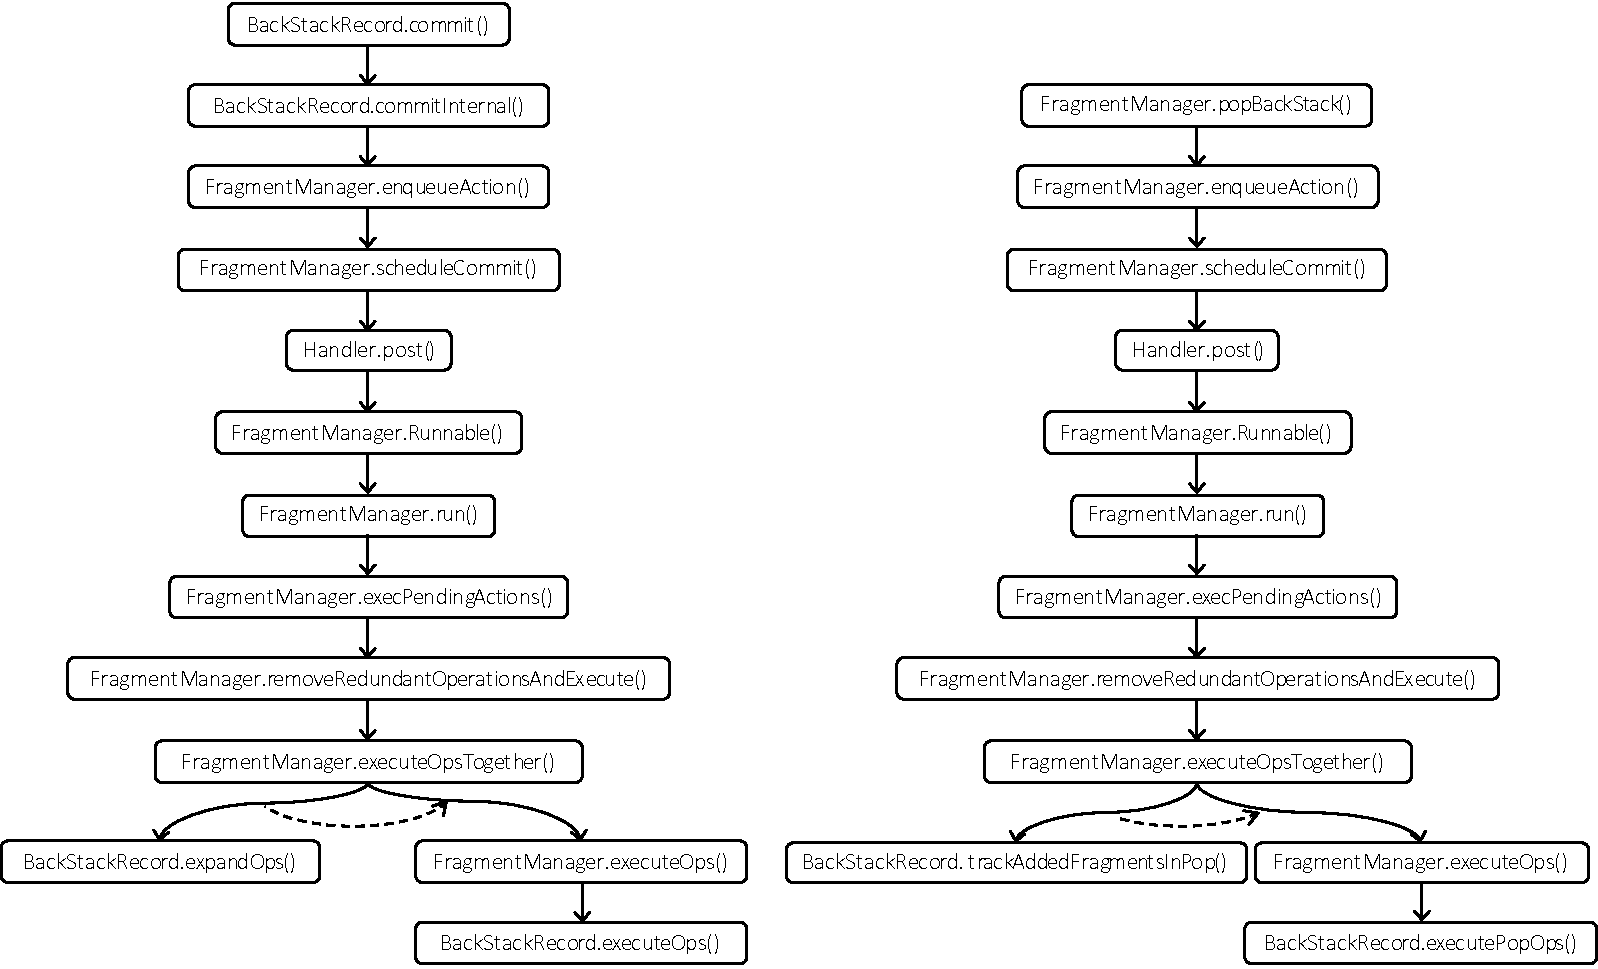
\includegraphics[scale = 0.55]{commit.pdf}
        \caption{Call graphs for committing and popping a fragment transaction}
            %in $\phi$
    % \vspace{-6mm}	
    \label{fig:commit}
\end{figure}

The control flows of committing and popping a fragment transaction are illustrated in Figure~\ref{fig:commit}. 
\begin{itemize}
\item We start with committing a fragment transaction first. From Figure~\ref{fig:commit}, to commit a fragment transaction, commit() is called. Then it calls commitInternal(), which calls enqueueAction() and so on  until executeOpsTogether() is called, where the core control logic for committing a fragment transaction is implemented. The procedure executeOpsTogether() calls expandOps() first, then executeOps(). Finally, executeOps() calls BackStackRecord.executeOps(). 
%
\item The call graph for popping a fragment transaction is similar. From Figure~\ref{fig:commit}, to pop a fragment transaction, popBackStack() is called. Then it calls commitInternal(), which calls enqueueAction() and so on  until executeOpsTogether() is called. The procedure executeOpsTogether() calls trackAddedFragmentsInPop() first, then executeOps(). Finally, executeOps() calls BackStackRecord.executePopOps(). 
\end{itemize}

We audit the source codes of the procedure executeOpsTogether() as well as those called by it directly or indirectly and confirm that 
\begin{itemize}
\item the way of dealing with REP actions in the semantics of $\FOAMASS$ in Section~\ref{sec-foamass} is consistent with the source code of expandOps(), 
\item the execution of fragment actions as defined in the semantics of $\FOAMASS$ in Section~\ref{sec-foamass} is consistent with the source code of BackStackRecord.executeOps(),
\item the way of revoking fragment transactions in the semantics of $\FOAMASS$ in Section~\ref{sec-foamass} is consistent with the source code of trackAddedFragmentsInPop(). 
\end{itemize}
The details of the auditing are relegated to Appendix~\ref{app:code-audit-fomass}.


%%%%%%%%%% original texts by Jinlong
%%%%%%%%%% original texts by Jinlong
\hide{
Moreover, from line 914 to line 932, the "remove" action of each fragment from the fragment stack will be pushed into fragment transaction sequentially, and the "add" action will be pushed into the fragment transaction in line 932.

As shown in Code~\ref{code-execute}, expandOps() is used to expand the fragment transaction, executeOps() is used to execute the fragment actions sequentially of the expanded fragment transaction, Moreover,
\begin{itemize}
    \item expandOps() function expands the fragment transaction by converting the fragment action "replace" into a sequence of fragment actions, consisting only of "add" and "remove" actions. Moreover, from line 914 to line 932, the "remove" action of each fragment from the fragment stack will be pushed into fragment transaction sequentially, and the "add" action will be pushed into the fragment transaction in line 932.
    Therefore, it is consistent with our formal semantics of $\REP$ of $\FOAMASS$.
    \item executeOps() function executes the fragment actions sequentially of the expanded fragment transaction. From line 768 to line 775, we can see that it only executes the "add" and "remove" actions, since there is no "replace" action in the fragment transaction which is expanded by expandOps() function. Moreover, it push (resp. remove) the fragment into (resp. from) the fragment stack when executing "add" (resp. "remove") action in line 770 (resp. 774).
    Therefore, it is consistent with our formal semantics of $\ADD$ and $\REM$ of $\FOAMASS$.
\end{itemize}

We confirm the behavior of the fragment stack and fragment transaction back stack is consistent with our formal semantics of $\FOAMASS$ defined in Section~\ref{sec-foamass} by reviewing the Android source code. As shown in Code~\ref{scode-fragtran}, commit() function is involved to execute the fragment transaction $ft$, Code~\ref{code-commit} shows a series of function calls to respond to function commit(). Moreover,
\begin{itemize}
    \item in the BackStackRecord.java file, commit() function calls the commitInternal() function in line 646, then commitInternal() function calls enqueueAction() function of FragmentManager class in line 688.
    \item in the FragmentManager.java file, enqueueAction() function defined in line 1903 calls scheduleCommit() function in line 1919, then scheduleCommit() function calls post(mExecCommit) function to call Runnable() function in line 739, then it calls execPendingActions() function in line 743, then execPendingActions() function calls removeRedundantOperationsAndExecute() function in line 2067, then it calls executeOpsTogether() function in line 2166. Finally executeOpsTogether() function calls expandOps()  function of BackStackRecord class in line 2193 and executeOps() function in line 2205 which calls executeOps() function of BackStackRecord class in line 2410.
\end{itemize}
Consequently, there are two functions of BackStackRecord class, i.e., expandOps() and executeOps() responding the commit() function.

Furthermore, $\back$ action will cancel the effects of the top fragment transaction of the fragment transaction stack if stack is not empty. As shown in Code~\ref{code-commit}, the popBackStack() in FragmentManager.java will be involved, then it will call enqueueAction() function. Similarly, it will call executeOpsTogether() finally, the difference is that it will call trackAddedFragmentsInPop() function in line 2195 instead of expandOps() function. Moreover, when executeOpsTogether() calls the executeOps() function in line 2205, the parameters isRecordPop is set true, hence executeOps() function will call executePopOps() function in 2407 instead of executeOps(). As shown in Code~\ref{code-execute}, trackAddedFragmentsInPop() function will not convert any action, since there are only "add" and "remove" actions in the fragment transaction. The executePopOps() function will execute the reverse actions of the fragment actions in the fragment transaction sequentially, for example, it will execute "remove" (resp. "add") action, if there is a "add" (resp. "remove") action in the fragment transaction. In this way, the effects of the fragment transaction will be cancelled which is consistent with our formal semantics of $\FOAMASS$.

Therefore, through reviewing Android source code, we discover that the behavior of the fragment stack and fragment transaction stack shown in the source code is essentially consistent with the formal semantics of $\FOAMASS$.

\begin{lstlisting}[caption={The sample code for FragmentTransaction},label={scode-fragtran}]
    Fragment F1 = new Fragment1();
    Fragment F2 = new Fragment2();
    FragmentTransaction ft = getFragmentManager().beginTransation();
    ft.add(R.id, F1);
    ft.replce(R.id, F2);
    ft.remove(F2);
    ft.addToBackStack("");
    ft.commit();
\end{lstlisting}
%
\begin{lstlisting}[caption={Android source code for responding add(), replace(), remove() and addToBackStack()},label={code-add}]
// core/java/android/app/BackStackRecord.java
173     final class BackStackRecord extends FragmentTransaction implements
174             FragmentManager.BackStackEntry, FragmentManagerImpl.OpGenerator {
            ...
413         public FragmentTransaction add(int containerViewId, Fragment fragment) {
414             doAddOp(containerViewId, fragment, null, OP_ADD);
                ...
416         }
            ...
423         private void doAddOp(int containerViewId, Fragment fragment, String tag, int opcmd) {
                ...
455             fragment.mContainerId = fragment.mFragmentId = containerViewId;
                ...
458             addOp(new Op(opcmd, fragment));
459         }
            ...
465         public FragmentTransaction replace(int containerViewId, Fragment fragment) {
                ...
470             doAddOp(containerViewId, fragment, tag, OP_REPLACE);
                ...
472         }
            ...
474         public FragmentTransaction remove(Fragment fragment) {
475             addOp(new Op(OP_REMOVE, fragment));
                ...
478         }
            ...
555         public FragmentTransaction addToBackStack(String name) {
                ...
560             mAddToBackStack = true;
                ...
563         }
            ...
1024    }
\end{lstlisting}

\begin{lstlisting}[caption={Android source code for responding commit() and popBackStack()},label={code-commit}]
// +/master/core/java/android/app/BackStackRecord.java
645     public int commit() {
646         return commitInternal(false);
647     }

// +/master/core/java/android/app/BackStackRecord.java
671     int commitInternal(boolean allowStateLoss) {    
            ...
683         if (mAddToBackStack) {
684             mIndex = mManager.allocBackStackIndex(this);    
                ...
687         }
688         mManager.enqueueAction(this, allowStateLoss);    
        ...
690     }

// +/master/core/java/android/app/FragmentManager.java
739     Runnable mExecCommit = new Runnable() {
740         @Override
741         public void run() {
742             execPendingActions();
743         }
744     };

// +/master/core/java/android/app/FragmentManager.java
828     public void popBackStack() {
829     enqueueAction(new PopBackStackState(null, -1, 0), false);
830     }

// +/master/core/java/android/app/FragmentManager.java
1903    public void enqueueAction(OpGenerator action, boolean allowStateLoss) {
            ...
1919        scheduleCommit();
            ...
1921    }

// +/master/core/java/android/app/FragmentManager.java
1929    private void scheduleCommit() {
            ...
1936        mHost.getHandler().post(mExecCommit);
            ...
1939    }

// +/master/core/java/android/app/FragmentManager.java
2060    public boolean execPendingActions() {
            ...
2067        removeRedundantOperationsAndExecute(mTmpRecords, mTmpIsPop);
            ...
2078    }

// +/master/core/java/android/app/FragmentManager.java
2128    private void removeRedundantOperationsAndExecute(ArrayList<BackStackRecord> records,
2129            ArrayList<Boolean> isRecordPop) {
            ...
2166        executeOpsTogether(records, isRecordPop, startIndex, numRecords);
            ...
2168    }

// +/master/core/java/android/app/FragmentManager.java
2178    private void executeOpsTogether(ArrayList<BackStackRecord> records,
2179            ArrayList<Boolean> isRecordPop, int startIndex, int endIndex) {
            ...
2192        if (!isPop) {
2193            oldPrimaryNav = record.expandOps(mTmpAddedFragments, oldPrimaryNav);
2194        } else {
2195            record.trackAddedFragmentsInPop(mTmpAddedFragments);
2196        }
            ...
2205        executeOps(records, isRecordPop, startIndex, endIndex);
            ...
2236    }

// +/master/core/java/android/app/FragmentManager.java
2397    private static void executeOps(ArrayList<BackStackRecord> records,
2398            ArrayList<Boolean> isRecordPop, int startIndex, int endIndex) {
            ...
2402        if (isPop) {
                ...
2407            record.executePopOps(moveToState);
2408        } else {
                ...
2410            record.executeOps();
2411        }
            ...
2413    }

\end{lstlisting}
}
%%%%%%%%%% original texts by Jinlong
%%%%%%%%%% original texts by Jinlong



\subsection{Empirical validation of the formal semantics}\label{sec:val-exp}
\revision{
The goal of this section is to validate the formal semantics empirically by comparing the actual behaviors of Android apps with their expected behaviors according to the formal semantics of the $\AMASS$ models that are extracted from them. To ease the empirical validation, we try to automate the process and propose a partially automated method for semantics validation in the sequel, by utilizing the nuXmv model checker, the Android UIAutomator testing framework, and the ADB tool. 
%Therefore, we propose an automated method %of automatically validating the formal semantics 
%by utilizing %the symbolic model checker 
%the nuXmv model checker, the Android UIAutomator testing framework, and the ADB tool. 
}

\paragraph*{Partially automated method for semantics validation}
%
Let $X$ be an Android app and $\Mm$ be an $\AOAMASS$ (resp. $\FOAMASS$) model that is extracted from $X$ and $\Aa$ be the nuXmv FSM model that encodes the configuration reachability problem of $\Mm$, where $c_t$, the bound on the number of tasks of the same affinity, and $\hbar$, the bound on the height of the stacks, are set to be $2$ and $6$ respectively. 
%We let $c_t  = 2$ and $\hbar = 6$ here, since in this case we assume that there is no fragments in activity, hence we have $k_a=0$. 
Moreover, $k_a$, the number of actions in one fragment transaction, is set to be $2$. 
%With the bounds $c_t, k_a, \hbar$, $\Mm$ is encoded by a nuXmv FSM model $\Aa$. 


The partially automated method to validate the semantics goes as follows. For a transition rule $\tau$ in $\Mm$,  
\begin{enumerate}
\item we use nuXmv to search for a path $\pi = \pi_1 \cdots \pi_m$ in $\Aa$, where an accepting condition corresponding to $\tau$ is set, in order to reach a configuration where $\tau$ can be applied (in other words, $\tau$ is enabled by the configuration), 
%that $A$ is the top activity of $S_1$, there is $i$ such that $i \neq 1$, $A_i = B$ and $i$ is the minimum such index, moreover, $B$ occurs in $S_i$ and $B$ is not the top activity of $S_i$ and $\zeta_i \neq \mainflag $. 
%
\item we generate from the app $X$ and each transition $\pi_i$ with $i \in [m]$, a sequence of click events in $X$, say $e_i$,
%
\item we use UIAutomator to execute the click events in $e_1, \cdots, e_m$ one by one (the task stack is updated), moreover, after the execution of all the click events, we use ADB to extract the resulting configuration, that is, the contents of the resulting task stack, say $\rho$,  

\item we generate the sequence of click events in $X$, say $e$, to fulfill the application of the transition rule  $\tau$,   
%
% \item Then for each $\phi \models \neg \tohflag \wedge \ntkflag \wedge \neg \mtkflag \wedge \rtfflag \wedge \neg \ctpflag \wedge \neg \ctkflag $, namely, for $\phi_0 = \neg \tohflag \wedge \ntkflag \wedge \neg \mtkflag \wedge \rtfflag \wedge \neg \ctpflag \wedge \neg \ctkflag \wedge \neg \stpflag$ and $\phi_1 = \neg \tohflag \wedge \ntkflag \wedge \neg \mtkflag \wedge \rtfflag \wedge \neg \ctpflag \wedge \neg \ctkflag \wedge \stpflag$, we generate two sequences of click events, say $e'_0, e'_1$, for two transition rules $\tau_0 = A \xrightarrow{\startactivity(\phi_0)} B$ and $\tau_1 = A \xrightarrow{\startactivity(\phi_1)} B$, that describe the selection of the launch mode and task affinity of $B$, the check boxes for intent flags, the FinishActivity option, and finally the operation of clicking the ``START ACTIVITY'' button.  
%
% \item We use UIAutomator again to execute the click events in $e'_0$ (resp. $e'_1$) one by one, and use ADB to obtain the resulting configuration $\rho'_0$ (resp. $\rho'_1$). Let $\tau_0(\rho)$ (resp. $\tau_1(\rho)$) denote the expected configuration obtained by applying $\tau'_0$ (resp. $\tau'_1$) on $\rho$ according to the formal semantics. If $\tau_0(\rho) \neq \rho'_0$ or $\tau_1(\rho) \neq \rho'_1$, then report that the formal semantics of {\AMASS} models and the actual semantics of Android multitasking mechanism are different. 
\item we use UIAutomator again to execute the click events in $e$ one by one, and use ADB to obtain the resulting configuration $\rho'$,
%
\item if $\rho' \neq \tau(\rho)$, then report the semantic inconsistency, where 
$\tau(\rho)$ denotes the expected configuration obtained by applying $\tau$ on $\rho$ according to the formal semantics. 
%If $\tau(\rho) \neq \rho'$, then report that the formal semantics of {\AMASS} models and the actual semantics of Android multitasking mechanism are different.
\end{enumerate}
\revision{Note that the generation of sequences of click events for transition rules (namely, the second and fourth step in the aforementioned procedure) is \emph{not} automated. 
For a transition rule of the form $\tau = A\xrightarrow{\alpha(\phi)} B$, we can click the widgets in the activity $A$  in order to find a sequence of click events so that the activity $B$ can be launched. Nevertheless, just from the sequence of click events and without the manual inspection of the source code, it is difficult, if not impossible, to figure out the intent flags associated with the action of starting the activity $B$ from the activity $A$. As a result, it is hard to determine that a sequence of click events corresponds to the transition rule $\tau$, even though we do know that the activity $B$ is started from $A$. }


%However, There maybe multiple sequences of click events to launch $B$, 
%making it difficult to automatically associate the correct sequence with the transition rule extracted from the app. 
%Hence, we need to audit the source code of the app to check which sequence is corresponding to the transition rule $\tau$. }
%Therefore, the semantics validation method is automated in the sense that it can automatically execute the sequences of click events and compare the resulting configurations, but the sequences of click events should still be \emph{manually} generated. 

\revision{Since generating sequences of click events for transitions is a manual process, it is hard to apply the aforementioned partially automated method for semantics validation to a large pool of Android apps from F-Droid or GooglePlay. As a result, in the sequel, we only select a small number of (more precisely, 20) apps from F-Droid to validate the formal semantics.
\begin{itemize}
\item At first, we select 10 apps to cover as many launch modes and intent flags as possible for validating the semantics of $\AOAMASS$. 
%
\item Then, we select 10 apps to cover as many types of fragment transactions as possible for validating the semantics of $\FOAMASS$.
\end{itemize}
We generate the sequences of click events from the transition rules by manually inspecting the source codes of these 20 apps.}
%, which also partially explains why we do not choose the commercial apps from GooglePlay to validate the formal semantics, since their source codes are unavailable.}  

Nevertheless, these 20 apps still do not cover the vast number of cases in the definition of the semantics of $\AOAMASS$ and $\FOAMASS$, since there are exponentially many different combinations of intent flags. Therefore, in addition to these apps, we design a special Android app ValApp\footnote{available at https://github.com/Jinlong-He/ValApp/tree/main}, aiming at covering all the cases in the definition of the semantics of $\AOAMASS$ and $\FOAMASS$ models. 

As a result, we mainly rely on ValApp to enumerate the different combinations of intent flags and carry out semantics validation for them.  
%
Note that this way %using ValApp to fulfill the semantics validation 
%does not affect very much the soundness 
is largely credible since, after the options (e.g. launch modes and intent flags) are chosen, the rest of the validation process is the same as real-world Android apps, that is, the startActivity() procedure is executed in the Android OS and the results are collected and compared. 


%This partially explains why we choose only 20 real-world apps to validate the semantics and mainly relies on ValApp to fulfill the validation. 

%We select 20 apps from F-Droid to validate the formal semantics. At first, we select 10 apps to cover as many launch modes and intent flags as possible for validating the semantics of $\AOAMASS$. Then we select 10 apps to cover as many types of fragment transactions as possible for validating the semantics of $\FOAMASS$.
%%%%%%%%%% original version. 
% To validate the semantics of $\AOAMASS$ empirically, we select 10 apps from F-Droid. These apps are selected to cover as many launch modes and intent flags as possible.  Similarly, to validate the semantics of $\FOAMASS$, we select 10 apps from F-Droid to cover as many types of fragment transactions as possible. 
%%%%%%%%%% original version. 

% \jinlong{the main reason is that the intent flags may interfere with each other. For example, $\ctpflag$ will be ignored when $\ctkflag$ is set, hence real world apps may not use $\ctkflag$ and $\ctpflag$ together. However, we need to validate all possible combinations of intent flags to ensure the correctness of the semantics of $\AOAMASS$, even though most combinations are not used in the real world apps.}

%The reason that we only select 10 real-world apps to validate the semantics of $\AOAMASS$ or $\FOAMASS$, instead of %validate the semantics by 
%	
%experimenting on a large pool of apps, in that %although we shall propose an automated method for semantics validation in Section~\ref{sec-aut-val}, 
%it is hard to apply the automated method to a large number of existing apps,  since generating sequences of click events for transitions is still a manual process \revision{(see Section~\ref{sec-aut-val})}. 
%As a result, we mainly rely on ValApp to carry out semantics validation. 
%
%Note that this way %using ValApp to fulfill the semantics validation 
%does not affect very much the soundness 
%is largely credible since, after the options (e.g. launch modes and intent flags) are chosen, the rest of the validation process is the same as real-world Android apps, that is, the %startActivity() procedure is executed in the Android OS and the results are collected and compared. 

\paragraph*{ValApp: A special Android app for the semantics validation.} A snapshot of ValApp is shown in Figure~\ref{fig:valapp}. ValApp includes 8 activities, corresponding to the $8$ (launch mode, task affinity) pairs from $\{\STD, \STP, \STK, \SIT\} \times \{1,2\}$. Moreover, ValApp provides means to choose the launch modes and intent flags, as well as ``start'' and ``finishStart'', so that transition rules can be generated for all their combinations. 
Furthermore, each activity of ValApp includes two fragments and two fragment containers. It also provides two variables for fragment identifiers and allows arbitrary combinations of actions to form fragment transactions. Finally, ValApp allows pushing arbitrarily many transactions into the fragment transaction stack. 
%
From the design, we can see that ValApp is capable of comprehensively accounting for all factors that may affect the semantics of $\AOAMASS$ and $\FOAMASS$ models. Moreover, ValApp is \emph{universal} in the sense that a user can interact with ValApp to choose the transition rules and generate a desired {\AMASS} model. 

%two fragment containers, for each activity. For each transition, ValApp can provide any combination of actions and combine them into fragment transactions of any length.

%two activities  each launch mode corresponds to two distinct activities with different affinities. For each transition, ValApp allows for any combination of intent flags and launch modes and the option to select "start" or "finishStart".
%ValApp also offers two fragments and two fragment containers for each activity. For each transition, ValApp can provide any combination of actions and combine them into fragment transactions of any length.

\begin{figure}[htbp]
\centering
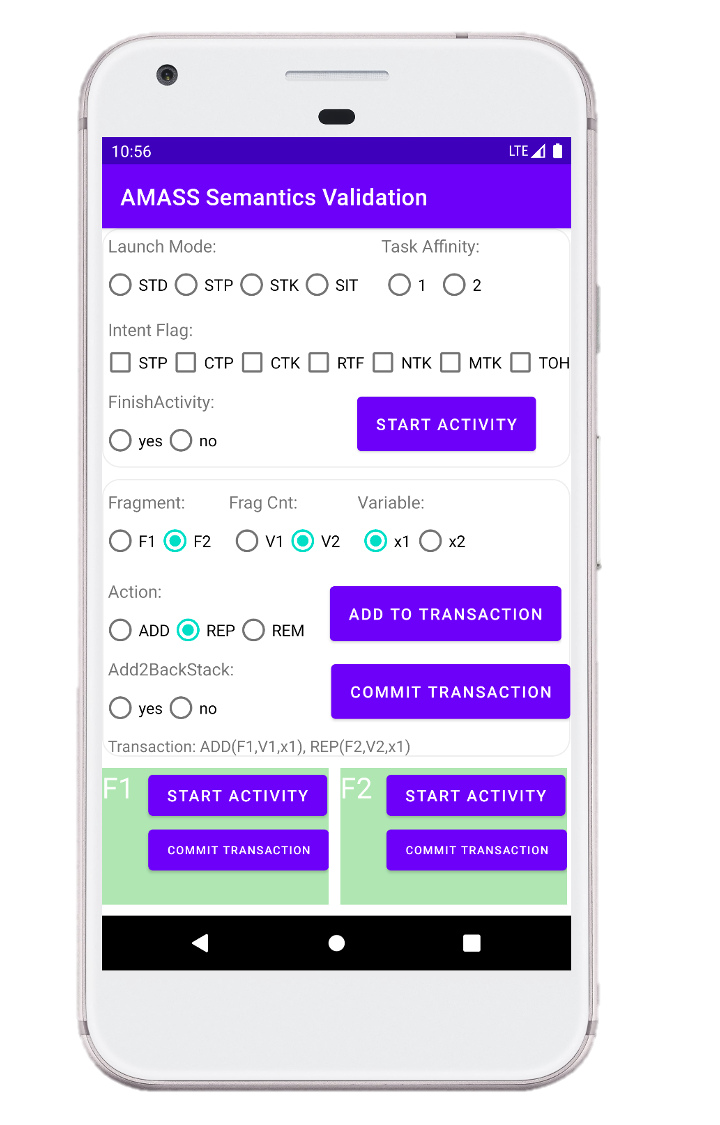
\includegraphics[scale=0.5]{ValApp.png}
\caption{ValApp: An Android app designed for validating the semantics of $\AMASS$}
\label{fig:valapp}
\end{figure}


%As shown in Figure~\ref{fig:valapp}, ValApp offers 8 selectable activities, where each launch mode corresponds to two distinct activities with different affinities. For each transition, ValApp allows for any combination of intent flags and launch modes and the option to select "start" or "finishStart".
%ValApp also offers two fragments and two fragment containers for each activity. For each transition, ValApp can provide any combination of actions and combine them into fragment transactions of any length.
%Therefore, by providing a range of selectable activities, different combinations of the intent flags, and customizable fragment transactions, ValApp is able to comprehensively account for all factors that may affect the semantics of the Android system.


%In this section, we validate the formal semantics of {\AMASS} models defined in Section~\ref{sec:amass} against the actual behavior of  Android apps.  To facilitate the validation, we selected $10$ apps from F-Droid , which cover as many launch modes, intent flags (resp. fragment transactions) as possible. (Note that we select apps from F-Droid because these open-source apps enable more accurate experimentation.)Because of the complicated  semantics, especially a vast number of possible combinations of launch modes and intent flags, real-world applications may not cover  all possible cases. To address this issue, we design an Android app “AMASS Semantics Validation” (abbreviated as ValApp) to facilitate the validation.

% Since the semantics are highly complicated, especially the number of the combinition of the launch modes and the intent flags is large, the real-world apps could not cover all the cases of the semantics, hence we design an Android app “AMASS Semantics Validation” (abbreviated as ValApp) to supplement the validation. 
% As shown in Figure 7, ValApp contains the following UI widgets.

% To facilitate the validation, we design an Android app   ``AMASS Semantics Validation'' (abbreviated as ValApp). 
%
%
% where radio buttons/check boxes for launch modes, task affinities, intent flags, fragments, fragment containers, and fragment transactions etc. are provided to generate the transition rules of {\AMASS} models. One the choices are made and a transition rule is generated, the transition rule can be executed by clicking the ``START ACTIVITY'' button or ``COMMIT TRANSACTION'' button, and the task stack will be updated. 
%
%
%Specifically, 
%As shown in Figure~\ref{fig:valapp}, ValApp offers 8 selectable activities, where each launch mode corresponds to two distinct activities with different affinities. For each transition, ValApp %allows for any combination of intent flags and launch modes and the option to select "start" or "finishStart".
%ValApp also offers two fragments and two fragment containers for each activity. For each transition, ValApp can provide any combination of actions and combine them into fragment transactions of any length.
%Therefore, by providing a range of selectable activities, different combinations of the intent flags, and customizable fragment transactions, ValApp is able to comprehensively account for all factors that may affect the semantics of the Android system.

% ValApp could apply any combinition of the launch modes and the intent flags for the transitions, 
% ValApp contains the following UI widgets.
%\hide{
%\begin{itemize}
%\item Eight activities, one for each pair (launch mode, task affinity), where the launch modes are from the set $\{\standard, \singletop, \singletask, \singleinstance\}$ and the task affinities are from $\{1, 2\}$. Moreover, it contains the following radio buttons and check boxes for the transition rules to start activities. 
%\begin{itemize}
%\item ValApp contains the radio buttons for choosing the launch modes and task affinities (1 or 2). Once the launch mode and task affinity are chosen, the activity of the corresponding launch mode and task affinity will be launched when the ``START ACTIVITY'' button is pressed. 
%%
%\item  ValApp contains eight check boxes, one for each intent flag, so that the intent flags can be configured to be valid or not. 
%%
%\item ValApp contains a radio button for choosing whether to finish the top activity or not, namely, whether a $\startactivity$ or $\finishstart$ transition rule will be executed. 
%\end{itemize}
%%
%\item ValApp contains two fragments $F_1, F_2$ and two fragment containers $V_1, V_2$. It also contains the following radio buttons for the transition rules to start fragment transactions.
%%
%\begin{itemize}
%\item ValApp contains the radio buttons for configuring fragment actions, i.e. the buttons for choosing $\{\ADD, \REP, \REM\}$, the fragments from $\{F_1, F_2\}$, the fragment containers from $\{V_1, V_2\}$, and the variables from $\{x_1, x_2\}$ to store the identifiers of fragment instances. Once a fragment action is configured, it can be added to a fragment transaction by clicking the ``ADD TO TRANSACTION'' button.
%%
%\item After adding all the actions to the current fragment transaction, the ``ASS2BackStack'' radio button can be used to choose whether to add the transaction into the fragment transaction stack.
%%
%\item When the configuration of a fragment transaction is complete, the ``COMMIT TRANSACTION'' button can be pressed to execute the actions in the transaction and update the fragment containers and fragment transaction stack. 
%%
%\end{itemize}
%\item Furthermore, the bottom of the ValApp window contains two copies of ``START ACTIVITY'' and ``COMMIT TRANSACTION'' buttons, corresponding to the transition rules of the form $F_i \xrightarrow{\alpha(\phi)} B$ and $F_i \xrightarrow{\mu} T$ ($i = 1,2 $).
%\end{itemize}
%}

%\tl{is this sentence finished?}
%Note that ValApp is a special app designated to do 

%Nevertheless, manual validation the formal semantics for all different cases and different Android versions is a daunting task. %, since the number of cases in the definition of the semantics is huge. Therefore, in the sequel, 
%Therefore, we propose an automated method %of automatically validating the formal semantics 
%by utilizing %the symbolic model checker 
%the nuXmv model checker, the Android UIAutomator testing framework, and the ADB tool. 

Let us focus on Android 13.0 in this section and validate the semantics of $\AOAMASS$ and $\FOAMASS$ models under this version. 
The verification of the formal semantics of $\AOAMASS$ and $\FOAMASS$  under the other versions is similar and omitted. 


%ValApp will be used as an example to describe the experiment. Then for each Android version from 7.0, 8.0, 9.0, 10.0, 11.0, 12.0, we validate the formal semantics against the actual behaviors of Android multitasking mechanism as follows. We enumerate all the cases in the semantics definition one by one, and for each case, validate the compatibility of the formal semantics with the actual behaviors of the ValApp. 

%\revision{Our semantics validation experiment is divided into three parts. Firstly, we validate the semantics of $\AOAMASS$ and $\FOAMASS$ separately. Then, we combine the above two experiments to validate the complete version of semantics.  }



%Note that in the aforementioned automated semantics validation method, the generation of sequences of click events in the app $X$ is manually done. As a result, 

%\revision{
\subsubsection{Validation of the formal semantics of $\AOAMASS$}
%
To valid the semantics, we consider the transition rules of the form $\tau = A\xrightarrow{\alpha(\phi)} B$, and generate one configuration for each combination of the launch modes of $A$ and $B$, the values of $\alpha$, the intent flags, and the constraints on the configuration before applying the transition, e.g. $\getrealtsk(\rho, B) = *$, $\gettsk(\rho, B) = S_1$, and $\topact(\rho) = B$. 
In total, there are $901,120$ different combinations to be considered and we would like to generate configurations for all of them.


%%%%%%%%%%%%%%%%%%%%%%%%%%%%%%%%%%%%%%%%%%%%%%%%%%%%%%%%%%%%
%%%%%%%%%%%%%%%%%%%%%%%%%%%%%%%%%%%%%%%%%%%%%%%%%%%%%%%%%%%%
\hide{
In order to validate semantics and avoid overfitting, we enumerated the launch modes of $A$ and $B$, the intent flags $\phi$ and the cases of the configurations $(\rho, b)$ where $\rho = ((S_1,A_1,\zeta_1),\cdots,(S_k,A_k,\zeta_k))$ for $\rho\xrightarrow[\tau]{\Mm}\rho'$ and $\tau = A\xrightarrow{\alpha(\phi)}B$.
\begin{enumerate}
    \item Launch modes: There are $4\times 4=16$ possible combinations of launch modes for $A$ and $B$. 
    % \item Start modes: There are $2$ cases of $\alpha$, i.e., $\startactivity$ and $\finishstart$.
    \item Intent flags: There are $2^{10}=1,024$ possible combination of the intent flags $\phi$.
    \item Configuration: According to the task allocation mechanism, we know there are $5$ cases,
    \begin{itemize}
        \item $\getrealtsk(\rho, B) = S_1$ and $\zeta_1 = \mainflag$,
        \item $\getrealtsk(\rho, B) = S_i$, $i > 1$ and $\zeta_i = \mainflag$,
        \item $\getrealtsk(\rho, B) = S_1$ and $\zeta_1 \neq \mainflag$,
        \item $\getrealtsk(\rho, B) = S_i$, $i > 1$ and $\zeta_i \neq \mainflag$,
        \item $\getrealtsk(\rho, B) = * \wedge \gettsk(\rho, B) = S_1$,
        \item $\getrealtsk(\rho, B) = * \wedge \gettsk(\rho, B) = S_i$, $i > 1$,
        \item $\gettsk(\rho, B) = *$,
    \end{itemize}
    and for the first six cases, there are $3$ subcases for the existence of $B$, i.e., $B$ is the top activity, $B$ occurs in the task but not the top activity, $B$ dose not occur in the task. 
    % Moreover, For the first two case, we need consider whether the task is the main task or not, 
    Hence there are $3\times 6 + 1 = 19$ cases of the configurations. 
    % Note that when $\lmd(B) = \SIT$, there are only 7 cases of the configurations, since for each case, there is only one subcase for the existence of $B$, for the first four cases $B$ is the top activity, for the fifth and sixth case $B$ dose not occur in the task. Moreover, when $\lmd(A) = \SIT$, 
\end{enumerate}
Moreover, when $\lmd(A) = \SIT$ or $\lmd(B) = \SIT$, the existence of $B$ of the task is different. More specifically, 
\begin{itemize}
    \item when $\lmd(B) = \SIT$ and $\lmd(A) \neq \SIT$, there are only 4 cases of the configurations, since $\getrealtsk(\rho, B) = S_1$ or $\gettsk(\rho,B) = S_1$ cannot be satisfied, additionally the existence of $B$ in the task is only one case.
    \item when $\lmd(A) = \SIT$ and $\lmd(B) \neq \SIT$, there are only $3\times 3 + 1 = 10$ cases of the configurations, since $\getrealtsk(\rho, B) = S_1$ or $\gettsk(\rho,B) = S_1$ cannot be satisfied.
    \item when $\lmd(A) = \SIT$ and $\lmd(B) = \SIT$, there are only $7$ cases of the configurations, since for each case of the task allocation mechanism, there is one subcase for the existence of $B$.
\end{itemize}
there are $2$ cases of $\alpha$ (resp. $b$), therefore, there are 
$2\times 2\times 1,024 \times (9 \times 19 + 3 \times 4 + 3 \times 10 + 7) = 901,120$
% $9\times 2\times 2\times 1,024\times 19 + 3\times 2\times 2 \times 1024 \times 4 =1,245,184$
 different cases.
}
%%%%%%%%%%%%%%%%%%%%%%%%%%%%%%%%%%%%%%%%%%%%%%%%%%%%%%%%%%%%
%%%%%%%%%%%%%%%%%%%%%%%%%%%%%%%%%%%%%%%%%%%%%%%%%%%%%%%%%%%%

We utilize the 10 apps selected from F-Droid as well as ValApp to generate the configurations. The 10 F-Droid apps are selected to cover as many launch modes and intent flags as possible. The sizes of these apps, the number of activities and transition rules of the  $\AOAMASS$ models constructed out of these apps (i.e. $|\act|$ and $|\Delta|$), as well as the number of generated configurations can be found in Table~\ref{tab-val-act}. 
%As shown in Table~\ref{tab-val-act}, the 10 selected apps from F-Droid cover $6,231$ cases in total and ValApp covers all cases.  These experiments confirm the conformance of the (operational) semantics of $\AOAMASS$ in Section\ref{sec:amass} to the external behavior of the Android system.
\begin{table}[htbp]
    \centering
    \begin{tabular}{|c|c|c|c|c|}
    \hline
    \textbf{App (package name)} & size (MB) & $|\act|$ & $|\Delta|$ & \# configurations \\
    \hline
    com.fsck.k9 & 3.58 & $21$ & $76$ & $892$\\
    \hline
    org.andstatus.app & 3.37 & $12$ & $29$ & $203$\\
    \hline
    com.fsck.k9.material & 4.49 & $17$ & $53$ & $686$\\
    \hline
    org.videolan.vlc & 16.16 & $16$ & $36$ & $567$\\
    \hline
    com.github.kiliakin.yalpstore & 1.43 & $14$ & $119$ & $1,195$\\
    \hline
    one.librem.mail & 4.69 & $18$ & $74$ & $984$\\
    \hline
    one.librem.tunnel & 20.38 & $6$ & $34$ & $378$\\
    \hline
    eu.siacs.conversations.legacy & 11.12 & $17$ & $82$ & $993$\\
    \hline
    org.fdroid.k9 & 3.12 & $20$ & $70$ & $893$ \\
    \hline
    info.guardianproject.otr.app.im & 10.7 & $12$ & $43$ & $492$  \\
    \hline
    {\textbf{Total}} & - & - & - & $6,231$  \\
    \hline
    ValApp & - & $8$  & $131,072$ & $901,120$\\
    \hline
    \end{tabular}
    \caption{Validation of the formal semantics of $\AOAMASS$ for Android 13.0}
    \label{tab-val-act}
\end{table}
%
%We construct the $\AOAMASS$ models out of these apps. 
In the end, we generate $6,231$ configurations out of the F-Droid apps and $901,120$ configurations out of ValApp. Then we use these configurations to validate the formal semantics. Through experiments, we discover that for every combination, the configuration obtained by applying the transition rule corresponding to the combination according to the formal semantics and the actual configuration returned by ADB are equal, thus the formal semantics of $\AOAMASS$ for Android 13.0 are confirmed to be consistent with the actual behaviors of Android apps.  

%To validate the semantics of $\AOAMASS$, we select 10 apps from F-Droid, whose statistics can be found in Table~\ref{tab-val-act}. These apps are selected to cover as many launch modes and intent flags as possible. Moreover, we build the $\AOAMASS$ models out of these apps. 

%It turns out that these 10 $\AOAMASS$ models cover $6,231$ cases in the definition of the semantics of $\AOAMASS$. Nevertheless, 

%Moreover, we also use ValApp 

%\vspace{-4mm}

%%%%%%%%%%%%%%%%%%%%%%%%%%%%%%%%%%%%%%%%%%%%%%%%%%
%%%%%%%%%%%%%%%%%%%%%%%%%%%%%%%%%%%%%%%%%%%%%%%%%%
\hide{
To utilize the nuXmv tool in the semantics validation, we impose a bound $c_t$ on the number of tasks of the same affinity and a bound $\hbar$ on the height of the stacks. We let $c_t  = 2$ and $\hbar = 6$ here, since in this case we assume that there is no fragments in activity, hence we have $k_a=0$. With the bounds $c_t, k_a, \hbar$, the {$\AOAMASS$} model of an Android app is encoded by a nuXmv FSM model $\Aa$. 

We will use the following case to illustrate the process of the automated validation: 
$A \xrightarrow{\startactivity(\phi)} B$, $\lmd(A) = \lmd(B) = \STD$, $\phi \models \neg \tohflag\wedge \ntkflag \wedge \ndmflag \wedge \neg \mtkflag \wedge \rtfflag \wedge \neg \ctpflag \wedge \neg \ctkflag\wedge \stpflag \wedge\neg \pitflag\wedge\neg\nohflag$, $b = \neg \nohflag$, $\getrealtsk(\rho, B) = S_i$, $i \neq 1$, $\zeta_i \neq \mainflag$, $B \in S_i$ and $B \neq \topact(S_i)$ which is the subcase of the semantics we defined,
$\tau=A \xrightarrow{\startactivity(\phi')} B$, $\phi' \models \neg \tohflag$,  $\lmd(B) = \standard$, $\phi' \models \ndmflag \wedge\neg \mtkflag$,  $\getrealtsk(\rho, B) = S_i$, $i\neq 1$, $\phi' \models \neg \ctkflag$, $B \in S_i$. 
Note that $A$ and $B$ are from the eight activities in the ValApp.
\begin{enumerate}
\item At first, we use nuXmv to generate a path $\pi = \tau_1 \cdots \tau_m$ in $\Aa$ that leads the initial configuration to a configuration (state) $\rho = ((S_1,A_1,\zeta_1), \cdots, (S_n, A_n, \zeta_n))$ satisfying that $A$ is the top activity of $S_1$, there is $i$ such that $i \neq 1$, $A_i = B$ and $i$ is the minimum such index, moreover, $B$ occurs in $S_i$ and $B$ is not the top activity of $S_i$ and $\zeta_i \neq \mainflag $. 
%
\item Then we generate from the ValApp and each $\tau_i$ in $\pi$, a sequences of click events $e_i$, that describes the selection of the radio buttons/check boxes and the operation of clicking the ``START ACTIVITY'' button. 
%
\item We use UIAutomator to execute the click events in $e_1, \cdots, e_m$ one by one (the task stack is updated). Moreover, after the execution of all the click events, we use ADB to extract the resulting configuration, that is, the resulting contents of the task stack, say $\rho$. 

\item Then we generate the sequence of click events, say $e$, for the transition rule $A \xrightarrow{\startactivity(\phi)} B$, that describe the selection of the launch mode and task affinity of $B$, the check boxes for intent flags, the FinishActivity option, and finally the operation of clicking the ``START ACTIVITY'' button.  
%
% \item Then for each $\phi \models \neg \tohflag \wedge \ntkflag \wedge \neg \mtkflag \wedge \rtfflag \wedge \neg \ctpflag \wedge \neg \ctkflag $, namely, for $\phi_0 = \neg \tohflag \wedge \ntkflag \wedge \neg \mtkflag \wedge \rtfflag \wedge \neg \ctpflag \wedge \neg \ctkflag \wedge \neg \stpflag$ and $\phi_1 = \neg \tohflag \wedge \ntkflag \wedge \neg \mtkflag \wedge \rtfflag \wedge \neg \ctpflag \wedge \neg \ctkflag \wedge \stpflag$, we generate two sequences of click events, say $e'_0, e'_1$, for two transition rules $\tau_0 = A \xrightarrow{\startactivity(\phi_0)} B$ and $\tau_1 = A \xrightarrow{\startactivity(\phi_1)} B$, that describe the selection of the launch mode and task affinity of $B$, the check boxes for intent flags, the FinishActivity option, and finally the operation of clicking the ``START ACTIVITY'' button.  
%
% \item We use UIAutomator again to execute the click events in $e'_0$ (resp. $e'_1$) one by one, and use ADB to obtain the resulting configuration $\rho'_0$ (resp. $\rho'_1$). Let $\tau_0(\rho)$ (resp. $\tau_1(\rho)$) denote the expected configuration obtained by applying $\tau'_0$ (resp. $\tau'_1$) on $\rho$ according to the formal semantics. If $\tau_0(\rho) \neq \rho'_0$ or $\tau_1(\rho) \neq \rho'_1$, then report that the formal semantics of {\AMASS} models and the actual semantics of Android multitasking mechanism are different. 
\item We use UIAutomator again to execute the click events in $e$ one by one, and use ADB to obtain the resulting configuration $\rho'$. Let $\tau(\rho)$ denote the expected configuration obtained by applying $\tau$ on $\rho$ according to the formal semantics. If $\tau(\rho) \neq \rho'$, then report that the formal semantics of {\AMASS} models and the actual semantics of Android multitasking mechanism are different. 
\end{enumerate}
}
%%%%%%%%%%%%%%%%%%%%%%%%%%%%%%%%%%%%%%%%%%%%%%%%%%
%%%%%%%%%%%%%%%%%%%%%%%%%%%%%%%%%%%%%%%%%%%%%%%%%%

% \subsubsection{Experimental result}



%In order to validate the semantics automatically, it is necessary to put 
%
\subsubsection{Validation of the formal semantics of $\FOAMASS$}
%
To valid the semantics, we consider the transition rules of the form $\tau = A \xrightarrow{\mu} T$ or $F \xrightarrow{\mu} T$. 
Note that according to the definition of semantics of $\FOAMASS$ in Section~\ref{sec-foamass}, the only requirement for the enablement of $A \xrightarrow{\mu} T$ or  $F \xrightarrow{\mu} T$ is that the top activity or fragment is $A$ or $F$. This requirement does not constrain the configurations very much. 
To validate the semantics of $\FOAMASS$, we fix the values of the following parameters and generate configurations as well as transition rules with these values.
\begin{itemize}
\item there is only one activity, say $A_0$, 
%
\item the number of containers associated with $A_0$ is $1$, 
%
\item the maximum number of transactions in the transaction stack is $1$, 
%
\item the maximum number of fragment actions in a transaction is $2$, 
%
\item the identifiers in (concretized) fragment actions in a transaction are from the set $\{1,2\}$.
% 
\end{itemize}
Note that the maximum number of fragments in a container is bounded by $\hbar = 6$ (i.e. the bound on the height of the stacks).  
In total, there are $4032$ different configurations to be considered. 
We generate the $4032$ configurations, construct $\FOAMASS$ models out of these apps, apply the transition rules in the models to the generated configurations to validate the semantics.

We utilize the 10 apps selected from F-Droid as well as ValApp to validate the semantics. 
The 10 F-Droid apps are selected to include as many fragments and fragment transactions as possible. Moreover, when constructing $\FOAMASS$ models out of the F-Droid apps, we restrict our attention to an activity whose number of fragments is the greatest in the app. For ValApp, since the number of actions in a transaction can be unbounded, we restrict our attention to the transition rules where the number of actions in a transaction is at most $2$. 
The sizes of these apps, the number of activities and transition rules of the $\FOAMASS$ models constructed out of these apps (i.e. $|\frag|$ and $|\Delta|$), and the average number of actions per transaction, as well as the number of generated (configuration, transition rule) pairs can be found in Table~\ref{tab-val-act}. 

%\zhilin{stopped here}
%We impose an upper bound $k_a$ on the number of actions in a transaction of the ValApp, because otherwise the number of actions in a transaction could be unbounded and the number of transactions would be infinite. Here we choose the bound $k_a$ to be $2$. Then the number of fragment transactions is $24^2 = 576$, since the number of fragment actions is $3 \times 2 \times 2 \times 2 = 24$ (3 actions, i.e., $\ADD$, $\REP$ and $\REM$, 2 fragments and 2 fragment containers). Therefore the number of transitions is $576\times 2\times 2 + 1 = 2,305$, corresponding to $5$ types of transitions, i.e., $A\xrightarrow{\opstack}T$, $A\xrightarrow{\nopstack}T$, $F\xrightarrow{\opstack}T$, $F\xrightarrow{\nopstack}T$ and $\back$.
%Due to the fact that the behavior of fragments is independent of the content of the fragment stack, we generate $20$ configurations, which the transaction stack is non-empty, randomly to validate. 
%Therefore there are $2,305\times 20 = 46,100$ different cases. 
% Recall that, in these case there are $5$ cases of $\tau$, i.e., $\tau = \back$, $\tau = A\xrightarrow{\opstack} T$, $\tau = A\xrightarrow{\nopstack}T$, $\tau = F\xrightarrow{\opstack}T$ and $\tau = F\xrightarrow{\nopstack}T$. Then for each case we select $20$ configurations to validate. 

%We will use the following case to illustrate the process of the automated validation: $\tau =A \xrightarrow{\opstack} T$, and we let the current configuration is $\rho$.
%Similarly, we use nuXmv to generate a path $\pi= \tau_1 \cdots \tau_m$ in $\Aa$ that leads the initial configuration to the configuration (state) $\rho$, then we generate a sequences of click events $e_i$ for each $\tau_i$ in $\pi$, then we use UIAutomator to execute the click events in $e_1, \cdots, e_m$ one by one. Finally we generate the sequence of click events, say $e$, for the transition rule $\tau$, and use UIAutomator to execute $e$, and use ADB to obtain the resulting configuration $\rho'$. If $\tau(\rho) \neq \rho'$, then report that the formal semantics of {\AMASS} models and the actual semantics of Android multitasking mechanism are different. 

%\revision{As shown in Table~\ref{tab-val-frag} , for each app we generate 20 configurations and validate each transition on these configurations. These experiments confirm the conformance of the (operational) semantics of $\FOAMASS$ in Section~\ref{sec:amass} to the external behavior of the Android system.}
%
\begin{table}
    \centering
    \begin{tabular}{|c|c|c|c|c|c|}
    \hline
    \textbf{App (package name)} & size(MB) & $|\frag|$ & $|\Delta|$ & $\begin{array}{c} {\bf average} \\ {\bf \#actions/transaction} \end{array}$ & \textbf{\#(config, trans)} \\
    \hline
    org.fox.ttrss & 1.15 & $9$ & $18$ & $1.2$ & $26,405$ \\
    \hline
    exa.lnx.a & 2.88 &  $10$ & $18$ & $1.0$ & $21,403$ \\
    \hline
    org.wordpress.android & 4.31 & $7$ & $19$ & $1.1$ & $7,028$  \\
    \hline
    de.geeksfactory.opacclient & 4.06 &  $4$ & $23$ & $1.0$ & $1,919$  \\
    \hline
    se.oandell.riksdagen & 2.66 &  $6$ & $23$ & $1.5$ & $31,012$  \\
    \hline
    com.secuso.privacyFriendlyCodeScanner & 1.62 &  $6$ & $24$ & $1.0$ & $28,425$  \\
    \hline
    com.igisw.openmoneybox & 9.04 & $9$ & $28$ & $1.9$ & $38,543$  \\
    \hline
    xyz.hisname.fireflyiii & 4.82 & $16$ & $33$ & $1.1$ & $64,160$  \\
    \hline
    org.anhonesteffort.flock & 4.22 & $8$ & $41$ & $1.0$ & $51,507$  \\
    \hline
    dulleh.akhyou.fdroid & 4.17 & $4$ & $126$ & $1.8$ & $84,602$ \\
    \hline
    {\textbf{Total}} & - & - & - & - & $355,004$  \\
    \hline
    ValApp & - & $2$ & $577$ & $2.0$ & $1,745,856$\\
    \hline
    \end{tabular}
    \caption{Validation of the semantics of $\FOAMASS$ models}
    \label{tab-val-frag}
\end{table}
In the end, we generate $4,032$ configurations for each of the F-Droid apps and ValApp. 
We also generate 577 transition rules for ValApp. 
Therefore, the total number of (configuration, transition rule) pairs for F-Droid apps are $355,004$, while the number for ValApp is $1,745,856$. 
Then for all these pairs, we apply the transition rules on the configurations to validate the formal semantics. Through experiments, we discover that for each configuration and each transition rule, the configuration obtained by applying the transition rule according to the formal semantics and the actual configuration returned by ADB are equal, thus the formal semantics of $\FOAMASS$ for Android 13.0 are confirmed to be consistent with the actual behaviors of Android apps.  

%At first, we construct the {\AMASS} model $\Mm$ corresponding to the ValApp. 

%%%%%%%%%%%%% the original texts by Jinlong %%%%%%%%%%%%%%
%%%%%%%%%%%%% the original texts by Jinlong %%%%%%%%%%%%%%
%\hide{
%For each transition rule, 
%\begin{enumerate}
%    \item We first use $\Aa_{\Mm}$ to generate a path $\pi = \tau_1\dots\tau_m$ resulting a configuration $\rho$ satisfying that the constraint corresponding to the case, according to the diagnosis app and $\pi$, we generate a sequence  $e_1,\dots,e_m$, where for each $i\in[m]$, $e_i$ is a sequence of click events.
%    \item Then we use an Android-app simulator called UIAutomator to execute the click-event sequences $e_1,\dots,e_m$ one by one.
%    \item According to $\tau$ of each case, 
%    \begin{itemize}
%        \item $\tau = A \xrightarrow{\alpha} (B, \phi)$ or $\tau = F \xrightarrow{\alpha} (B, \phi)$. For each possible value of the intent flags satisfying the constraint corresponding to the case, we generate a click-event sequence $e$ to launch activity $B$ according to $\tau$ and the possible value of the intent flags. Then we use UIAutomator to execute $e$. And the resulting configuration $\rho'$ is recorded.
%        \item $\tau = A \xrightarrow{\mu} (\beta_1(F_1, i_1), \cdots, \beta_k(F_k, i_k))$ or $\tau = F \xrightarrow{\mu} (\beta_1(F_1, i_1), \cdots, \beta_k(F_k, i_k))$. For each possible actions sequence which the length of sequence is 2, we generate a click-event sequence $e$ according to $\tau$ and the sequence. Then we use UIAutomator to execute $e$. And the resulting configuration $\rho'$ is recorded.
%    \end{itemize}
%\item Finally we check whether the resulting configuration $\rho'$ and the configuration $\rho''$ which evolved from $\rho$ are the same.
%\end{enumerate}
%
%We design a diagnosis app $\theapp$ as shown in Fig~\ref{fig:valapp} and conduct experiments to validate the formal semantics of AMASS against the actual behavior of the app under different multitasking mechanisms in Android 6.0, 7.0, 8.0, 9.0, 10.0, 11.0 and 12.0.
%%
%The diagnosis app has 8 activities and 2 fragments $F_1,F_2$. The names, launch modes and task affinities of these activities can be found in Table~\ref{tab-attribute}, i.e., $\lmd(D_1)=\standard$ and $\aft(D_1) = 1$.
%%where ``'' means the empty-string task affinity. 
%The main activity of the diagnosis app is $D_1$.
%Each activity has two fragment stacks $V_1,V_2$ to display different fragments.
%In each activity, we can choose one launch mode (resp. task affinity) in \textbf{Launch Mode} (resp. \textbf{Task Affinity}) and choose some intent flags in \textbf{Intent Flags} for launching an activity, \textbf{FinishActivity} is to choose whether finishing the current activity.
%After choosing these, we can press on the button \textbf{START ACTIVITY} to launch the activity.
%For starting a fragment transaction, in each activity we can choose one fragment (resp. fragment stack, action type) in \textbf{Fragment} (resp. \textbf{Frag Stack}, \textbf{Action}) to construct an action, and press on the button \textbf{ADD} to add this action into the fragment transaction, 
%then we can press on the button \textbf{START FRAGMENT} to start this fragment transaction,
%\textbf{Add2BackStack} is to choose whether adding this fragment transaction into back stack when start it.
%
%
%%There are 2 buttons START ACTIVITY and START FRAGMENT in each activity and fragment, 
%%we can press on the button START ACTIVITY (resp. START FRAGMENT) to start activity (resp. fragment transaction).
%%which we can press on the button START ACTIVITY to start the activity, i.e., $\standard\_1$ via choosing the Launch Mode $\standard$ and Task Affinity $1$ with choosen some Intent Flags, if we choose yes in FinishActivity, then 
%%We can press on the button ADD to add the action, i.e., $\ADD(F_1,1)$ via cho into fragment transaction.
%%one start part to start activity or fragment, and one options part to choose launch modes, affinities, intent flags and fragment transactions to start activity or fragment.
%%The start part has 4 start buttons $startActivity$ to start an activity, $finishActivity$ to start an activity and finish the current activity, $startFragments$ to start a fragment transaction and $startFragments\sharp$ to start a fragment transaction and add this transaction into transaction stack.
%%The options part has two radio buttons to choose the launch mode and task affinity, one checkbox to choose the intent flags, one radio button to choose a fragment $F$, one radio button to choose the fragment stack $V_i$, one radio button to choose whether $\ADD$ or $\REP$ this fragment $F$ into fragment stack $V_i$, one button to add this action $\ADD(F, i)$ to fragment transaction.
%%There are 2 fragments $F_1,F_2$ in the diagnosis app and there are 4 same start buttons as activity in each fragment.
%%For instance, for the transition $\tau = A \xrightarrow{\startactivity(\phi)} B$,
%%we could choose the activity $B$ via choosing the launch mode and affinity (Each activity has different launch mode or affinity), and choose the intent flags satisfying $\phi$, and press on the $startActivity$ button to start activity $B$ in the current activity $A$.
%
%In each case of the definition of the semantics of starting an activity, i.e., $\tau = A \xrightarrow{\startactivity(\phi)} B$, if a flag does not affect the semantics, then it is omitted in the constraints corresponding to the case. For instance, the $\ctpflag$ flag is omitted for the case $\lmd(B)=\singletask$. However, in the validation experiments, we still need to consider all the possible values of these flags in order to be exhaustive.
%In each case of the definition of the semantics of starting a fragment transaction, i.e., $\tau = A \xrightarrow{\mu} (\beta_1(F_1, i_1), \cdots, \beta_k(F_k, i_k))$, we need to consider all the possible actions sequences, but the length of the sequence is unlimited, hence we impose an upper bound $2$ on  the length of actions sequence, there are $2^3\times 2^3\times 2=128$ possible actions sequences.
%To validate the semantics of switching the task, i.e., $\tau = A \xrightarrow{\startactivity(\phi)} B, \lmd(B) = \singletask$, there is a function $\gettsk(\rho,B) = S_i$ to addresse the target task $S_i$, such that $i\in[n]$ is the minimum index satisfying $\aft(A_i) = \aft(B)$, if such an index $i$ exists; We need to design the configuration such that there exists some tasks with the same affinity $\aft(B)$ to validate the correctness of this function.  Hence we need to use $\mtkflag$ flag to launch multiple tasks with the same affinity.
%%
%%Therefore, the validation experiments are done in the following way: 
%
%We are going to have a more detailed description of the semantics validation algorithm in the sequel. The algorithm relies on the following functions related to the tools nuXmv, UIAutomator, and ADB (Android Debug Bridge).
%\begin{itemize}
%    \item $genPossibleFlags(\phi)$ generates a set of formulaes $fs = \{\phi'\mid \phi'\models\phi\}$,
%    \item $genPossibleTransactions()$ generates for a set of transactions $ts = \{\mu[( (\beta_1(F_1,i_1),(\beta_2(F_2,i_2))) )]\mid \mu\in\{\nopstack,\opstack\},\forall j\in\{1,2\}, \beta_j\in\{\ADD,\REP\},F_j\in\{F\_1,F\_2\},i_j\in\{1,2\}\}$,
%    \item $\nuxmv.genPath(\Mm, \psi)$ generates for a configuration $\rho$ satisfying the constraint $\psi$, a path $\pi = \tau_1 \cdots \tau_m$ in $\Aa_{\Mm}$,
%%
%%\item $Gator.genClickSeq(path)$ generates for a path $\pi = \tau_1 \cdots \tau_m$ of $\Aa_\Mm$, a sequence $(\tau_1, t_1, e_1) \cdots (\tau_m, t_m, e_m)$, where each $e_i$ is a click-event sequence,
%%
%\item $UIAutomator.click(e)$ executes the click-event sequence $e$ on $\theapp$, \\
%    $UIAutomator.pressBack()$ presses the back button on $\theapp$,\\
%    $UIAutomator.restart()$ restarts $\theapp$,
%%
%%\item $UIAutomator.isClickable(e)$ returns true if the click-event sequence $e$ is testable in the foreground activity of {\theapp},
%%
%%\item $UIAutomator.getClickEvents()$ returns the set of click events in the foreground activity of {\theapp},
%%
%%\item $ADB.getFragments$ returns all the foreground fragments (in the containers), $ADB.getTopActivity$ returns the top activity, and $ADB.getTasks$ returns the whole task stack. 
%\item $ADB.getTasks()$ returns the configuration of the whole task stack. 
%\end{itemize}
%
%The aforementioned semantics validation algorithm is presented as the procedure $SemanticsValidate()$ in Algorithm~\ref{alg-validate}, which uses 
%two global variables $\Mm$ and $semantics$, where $\Mm$ is the $\AMASS$ model of \ $\theapp$, and $semantics$ is the formal semantics of AMASS, which can be considered as the set of the tuple $(\psi,\phi,\tau,f)$, where $\psi$ is the constraint we defined in the semantics of AMASS without $\phi$, $\phi$ is the intent flag formulae, $f$ is the function evolving configuration, viz, if a configuration $\rho$ satisfying $\psi\wedge\phi$, when $\tau$ is executed, $f(\rho)$ is evolved.
%The procedure $SemanticsValidate()$ calls another procedure $Check()$, which tries to check whether the semantics is correct under the constraints $\psi\wedge\phi$.
%
%\begin{algorithm}[]
%  \SetAlgoLined
%%  \SetKwInOut{Input}{input}
%%  \Input{$\Mm = (\act, A_0,\frag, \vgr, \lmd, \aft,  \Delta)$}
%%  \KwResult{testcases}
%\small
%\ForEach{$(\psi, \phi, \tau, f) \in semantics$}{ 
%      $path$ $\leftarrow$ $nuXmv.genPath(\Mm, \psi)$\;
%      $clickSeq$ $\leftarrow$ $genClickSeq(path)$\;
%      \eIf{$Check(\phi, \tau, f, clickSeq) = False$}{
%          \Return $\false$\;
%      }{}
%  }
%  \Return $\true$\;
%%  (new\_teacases,$\Delta$,ignores) $\leftarrow$ Explore(click\_seq, depth, ignores, \{\})\;
%%  teacases $\leftarrow$ teacases.extend(new\_testcases)\;
%%    \textbf{return} teacases
%  \caption{$SemanticsValidate(\Mm,semantics)$}
%    \label{alg-validate}
%\end{algorithm}
%
%\begin{algorithm}[]
%  \SetAlgoLined
%%  \SetKwInOut{Input}{input}
%%  \Input{$\Mm = (\act, A_0,\frag, \vgr, \lmd, \aft,  \Delta)$}
%%  \KwResult{testcases}
%\small
%    \uIf{$\tau = A/F \xrightarrow{\startactivity} (B, \phi)$ }{
%        $fs$ $\leftarrow$ $genPossibleFlags(\phi)$\;
%              \ForEach{$\phi' \in fs$}{ 
%                  \ForEach{$ e \in clickSeq$}{ 
%                          $UIAutomator.click(e)$\;
%                      }
%                  $\rho$ $\leftarrow$ $ADB.getTasks()$\;
%                  $clickSeq$ $\leftarrow$ $genClickSeq([A/F \xrightarrow{\startactivity} (B, \phi')])$\;
%                  \ForEach{$ e \in clickSeq$}{ 
%                          $UIAutomator.click(e)$\;
%                      }
%                  $\rho'$ $\leftarrow$ $ADB.getTasks()$\;
%                  \eIf{$f(\rho) \neq \rho'$}{
%                      \Return $\false$\;
%                  }{
%                      $UIAutomator.restart()$\;
%                  }
%              }
%          
%         }{
%             \ElseIf{$\tau = A/F \xrightarrow{\mu} T$}{
%            $ts$ $\leftarrow$ $genPossibleTransactions()$\;
%                 \ForEach{$\mu[T'] \in ts$}{ 
%                  \ForEach{$ e \in clickSeq$}{ 
%                          $UIAutomator.click(e)$\;
%                      }
%                  $\rho$ $\leftarrow$ $ADB.getTasks()$\;
%                 $clickSeq$ $\leftarrow$ $genClickSeq([A/F\xrightarrow{\mu}T'])$\;
%                  \ForEach{$ e \in clickSeq$}{ 
%                          $UIAutomator.click(e)$\;
%                      }
%                  $\rho'$ $\leftarrow$ $ADB.getTasks()$\;
%                  \eIf{$f(\rho) \neq \rho'$}{
%                      \Return $\false$\;
%                  } {
%                      $UIAutomator.restart()$\;
%                  }
%              }
%             }
%         \Else {
%              \ForEach{$ e \in clickSeq$}{ 
%                      $UIAutomator.click(e)$\;
%                  }
%              $\rho$ $\leftarrow$ $ADB.getTasks()$\;
%              $UIAutomator.pressBack()$\;
%          $\rho'$ $\leftarrow$ $ADB.getTasks()$\;
%          \eIf{$f(\rho) \neq \rho'$}{
%              \Return $\false$\;
%          } {
%              $UIAutomator.restart()$\;
%          }
%         }
%     }
%  \Return $\true$\;
%%  (new\_teacases,$\Delta$,ignores) $\leftarrow$ Explore(click\_seq, depth, ignores, \{\})\;
%%  teacases $\leftarrow$ teacases.extend(new\_testcases)\;
%%    \textbf{return} teacases
%  \caption{$Check(\phi,\tau,f,clickSeq)$}
%    \label{alg-check}
%\end{algorithm}
%}
%%%%%%%%%%%%% the original texts by Jinlong %%%%%%%%%%%%%%
%%%%%%%%%%%%% the original texts by Jinlong %%%%%%%%%%%%%%

 
%
%, where each row of the tables presents the results for one case of the semantics definition. Specifically, in each row of the tables,  
%\begin{itemize}
%\item the ``Semantics'' column describes the conditions for the case, 
%%
%\item the ``True Flags'' (resp. ``False Flags'') column specifies the intent flags that has to be true (resp. false) in  the case, 
%%
%\item the ``Current configuration'' column specifies the current configuration,
%%
%\item the ``Transition'' column describes the caller and callee activity of the transition (resp. the caller activity and the fragment transaction), 
%%
%\item the configurations resulted from executing the transition rules on the current configuration for different Android versions are listed in the columns ``Result for Android x.0'' (where $x = 6, 7, 8, 9, 10, 11, 12$). 
%\end{itemize}
%Furthermore, if the results for different Android versions are different, then they are highlighted by the red color.  


%%%%%%%%%%%%%%%%%%%%%%%%%%
\hide{
\begin{table}[htb]
\centering
\caption{Attributes of activities of the diagnosis app}
\label{tab-attribute}
\begin{tabular}{|c|c|c|c|c|c|}
\hline
Name & Launch mode & Task affinity\\
\hline
$D_1$ & $\standard$ & 1 \\
\hline
$D_2$ & $\standard$ & 2 \\
\hline
$P_1$ & $\singletop$ & 1 \\
\hline
$P_2$ & $\singletop$ & 2 \\
\hline
$K_1$ & $\singletask$ & 1 \\
\hline
$K_2$ & $\singletask$ & 2 \\
\hline
$T_1$ & $\singleinstance$ & 1 \\
\hline
$T_2$ & $\singleinstance$ & 2 \\
\hline
\end{tabular}
\end{table}
\vspace{-4mm}
%
The experimental results can be found by unzipping the \textbf{supplementary material} and browsing 
%the Excel file semantics$\_$validation.xlsx or 
the web page semantics$\_$validation.htm, where 
\begin{itemize}
\item the ``Semantics'' column specifies the constraint for one case of the semantics, 
\item the ``Current configuration'' column gives the current configuration,
\item the ``Transition'' column gives the source activity or source fragment and target activity or $\mu$,
\item the ``True Flags'' (resp. ``False Flags'') column gives the intent flags that has to be set to true (resp. false) in that case, 
\item the ``Fragment Transaction'' column gives gives the actions sequence set in the current fragment transaction,
\item the columns ``Result for Android 6.0/7.0/8.0/9.0/10.0/11.0/12.0/13.0'' show the configurations obtained after executing the transition on the current configuration. 
\end{itemize}
Moreover, the results showing the differences of the semantics for Android 6.0, 7.0, 8.0, 9.0, 10.0, 11.0, 12.0 and 13.0 are highlighted by red/green colors.  
\hide{
%\vspace{-8mm}
\begin{table}[htb]
\centering
\caption{Attributes of activities of the diagnosis app}
\label{tab:attribute}
\begin{tabular}{|c|c|c|c|c|c|}
\hline
Name & Launch mode & Task affinity&Name & Launch mode & Task affinity \\
\hline
D_1 & $\standard$ & 1 & P_1 & $\singletop$ & 1\\
\hline
D_2 & $\standard$ & 2 & P_2 & $\singletop$ & 2\\
\hline
D_3 & $\standard$ & 3 & P_3 & $\singletop$ & 3\\
\hline
D & $\standard$ & ``'' & P & $\singletop$ & ``''\\
\hline
K_1 & $\singletask$ & 1 & T_1 & $\singleinstance$ & 1\\
\hline
K_2 & $\singletask$ & 2 & T_2 & $\singleinstance$ & 2\\
\hline
K_3 & $\singletask$ & 3 & T_3 & $\singleinstance$ & 3\\
\hline
K & $\singletask$ & ``'' & T & $\singleinstance$ & ``''\\
\hline
\end{tabular}
\end{table}
\vspace{-4mm}
}
}

%=================================================================================================






